\chapter{Diseño e implementación del servidor}

En este capítulo se explicará el diseño y la implementación del server. En la Fig. \ref{fig:server-final} se observa la versión final del servicio, mostrando la interacción entre los Clientes, los sistemas SL y el Server.

\begin{figure}[bth]
    \centering
    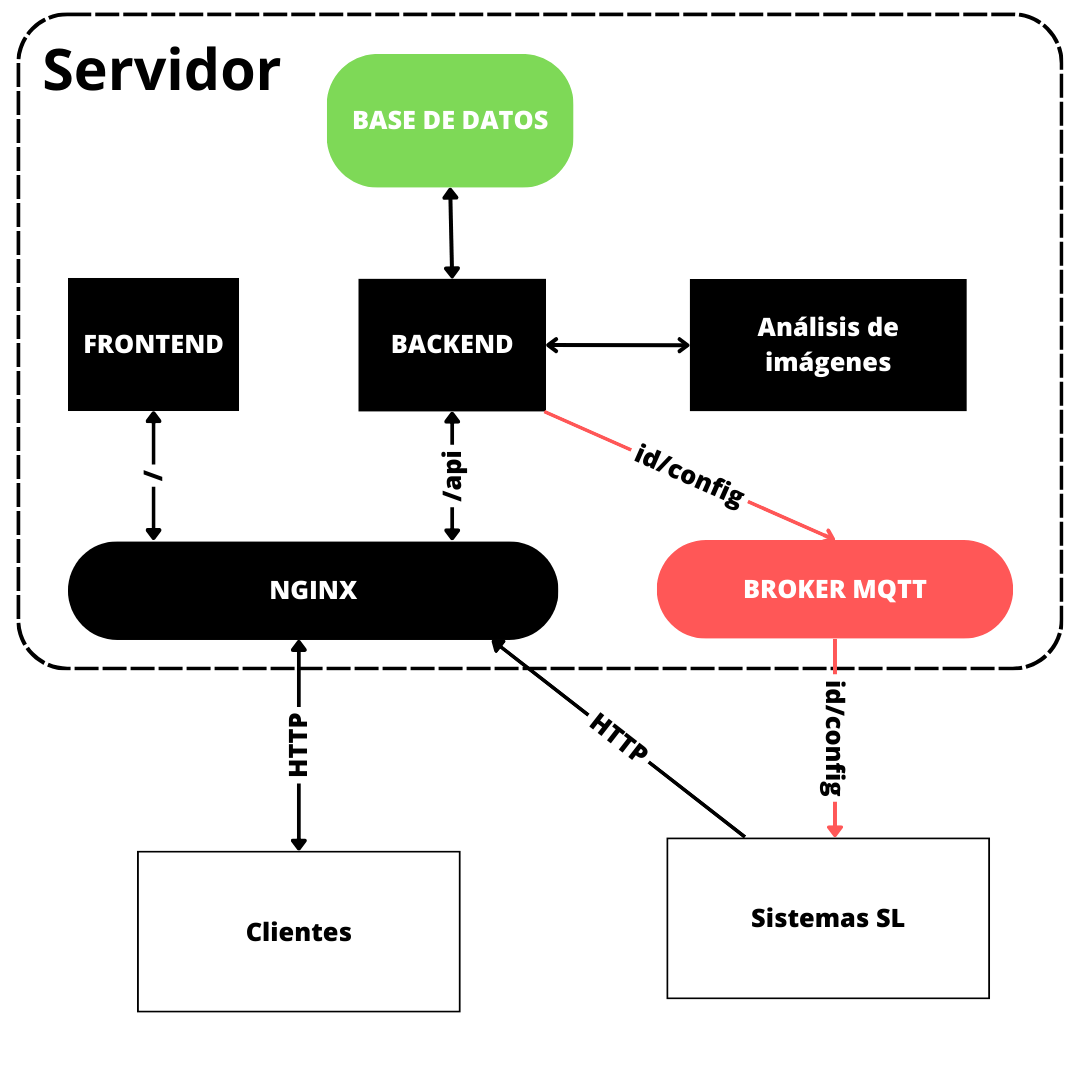
\includegraphics[width=.6\textwidth]{imgs/server-esquema.png}
    \caption{Esquema final del servidor.}
    \label{fig:server-final}
\end{figure}

\section{Actualidad del desarrollo web}

En la web existen dos grandes pilares: el front-end es la parte de la aplicación web con la que interactúan los usuarios o clientes. El back-end que es la parte que se conecta con la base de datos y ejecuta las validaciones necesarias para leer o escribir información. En general, el front-end y el back-end suelen ser dos proyectos separados y pueden ser construidos en diferentes lenguajes. Los lenguajes más utilizados para desarrollo back-end son: JavaScript (JS), Python, Ruby, entre otros \cite{presta_10_2021}.

En la actualidad el formato más utilizado para trasmitir información entre el back-end y el front-end es el formato JSON de sus siglas en inglés JavaScript Object Notation o traducido como notación de objetos de JavaScript. En la Fig. \ref{fig:ejemplo-json} se observa un ejemplo de JSON. Este tipo de notación se caracteriza por almacenar los datos en forma clave-valor, permitiendo un acceso a la información rápido y sencillo.

\begin{figure}[bth]
    \centering
    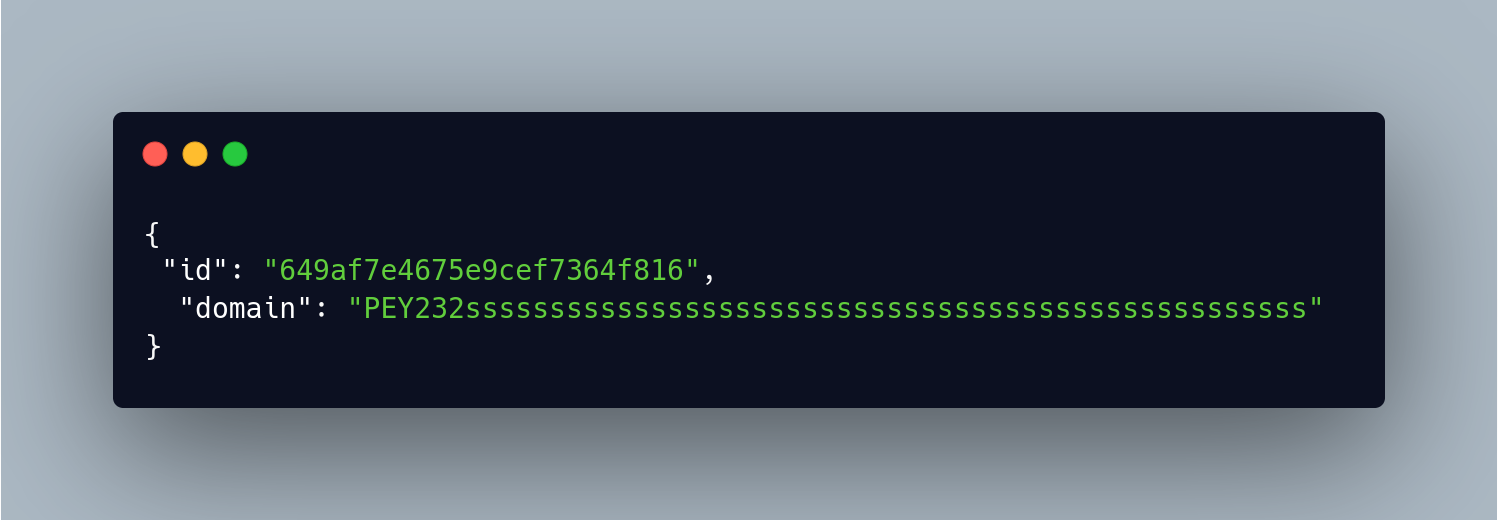
\includegraphics[width=.5\textwidth]{imgs/json-example.png}
    \caption{Ejemplificación de un JSON.}
    \label{fig:ejemplo-json}
\end{figure}

Hoy en día la web se ha transformado en la base de cualquier organización. Hace años las organizaciones solían usar aplicaciones de escritorio, pero en la actualidad las aplicaciones web han dominado el mercado.

\section{Docker}

Docker es una tecnología open source desarrollada por Docker Inc, la cual permite correr aplicaciones de forma aislada en contenedores.

\subsection{Contenedores}

Un contenedor funciona casi como una máquina virtual, pero sin entorno gráfico y compartiendo el Kernel \cite{keepcoding_que_2022} con el sistema que lo hospeda, lo que hace que los contenedores sean más livianos y mucho más rápidos que una máquina virtual, ya que estas últimas emulan todo el sistema e incluyen un puente entren el kernel del sistema padre y el sistema emulado. Cada contenedor suele estar especializado para cumplir una determinada tarea y, en general, se los denomina servicios.

\subsection{Docker Compose}

A pesar que Docker es una tecnología muy utilizada, por si sola puede ejecutar un único contenedor a la vez, existen herramientas para la administración de múltiples contenedores en simultáneo. La más conocida, y muy utilizada en el mundo del desarrollo es Kubernetes \cite{noauthor_kubernetes_nodate}.
Debido a que el sistema aun no es lo suficientemente grande y no se cuenta con múltiples servidores para alojar los servicios, la implementación se realizó mediante Docker Compose \cite{docker_inc_docker_2023}, cumple un rol muy similar a Kubernetes, pero sin agregar tanta complejidad debido a poder administrar múltiples servidores.

\begin{figure}[bth]
    \centering
    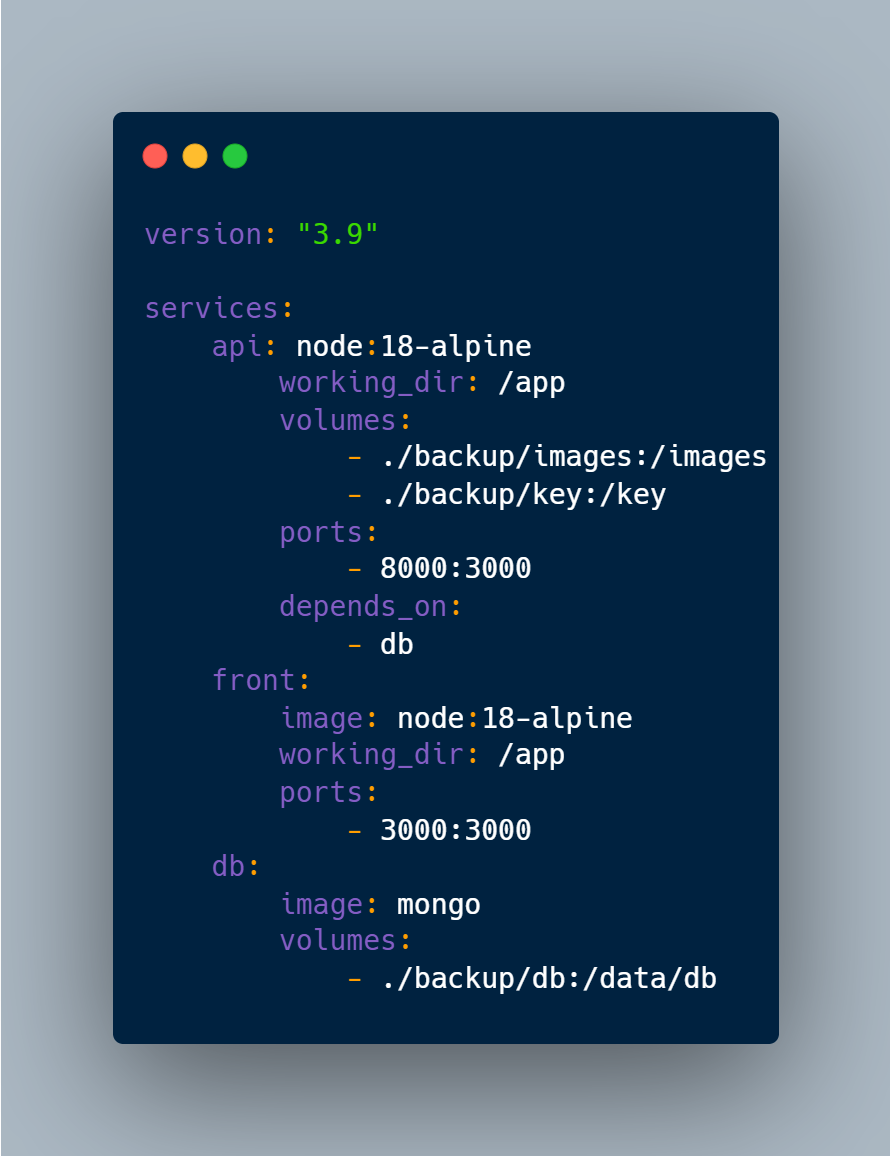
\includegraphics[width=.5\textwidth]{imgs/docker-compose.png}
    \caption{Ejemplificación de una archivo \textit{docker-compose.yml}}
    \label{fig:docker-compose-yml}
\end{figure}

El proceso de configuración de Docker Compose se hace creando un archivo de extensión YAML como el de la Fig. \ref{fig:docker-compose-yml}. Se puede observar que existen dos apartados principales.

\subsubsection{version}

Este atributo le indica a Docker Compose la versión del archivo de configuración que se está utilizando, en general, esta versión impacta directamente en qué atributos se pueden utilizar en el resto del archivo de configuración.

\subsubsection{services}

Se definen los servicios que se necesitarán. En la Fig. \ref{fig:docker-compose-yml} se muestran tres contenedores \textit{api}, \textit{front}, \textit{db}.

Dentro de cada contenedor se define el atributo \textit{image} el cual indica que imagen se utilizará. Dicha imagen puede ser privada o  se puede utilizar una imagen pública de Docker Hub que es un repositorio de imágenes de Docker.
Las imágenes son en esencia un sistema operativo configurado para algunos entornos, por ejemplo la imagen \textit{node:18-alpine} posee un sistema Alpine, que ya viene instalado con NodeJS en su versión 18, imagen muy utilizada para correr aplicaciones escritas en JS.

Otro campo que se destaca es el \textit{working\_dir} o directorio de trabajo, que es donde se almacenará el código de la aplicación. Es importante destacar que esta ruta se toma desde el contenedor, y no tiene por qué ser una ruta válida desde el sistema Host.

El atributo \textit{volumes} es un array que vincula una carpeta del sistema Host con una carpeta del contenedor, permitiendo acceder a la información del contenedor.
Esto es muy utilizado para realizar backup desde el sistema Host.

Por último, \textit{ports} es un array que vincula los puertos del sistema anfitrión a los puertos del contenedor, lo que es sumamente útil cuando se desea escuchar un puerto específico para manejar peticiones HTTP, por ejemplo.

\subsubsection{intranet}

Si bien en el archivo de configuración no aparece la configuración de \textit{intranet}, Docker Compose genera una red interna para interconectar los contenedores, lo que permite que el servicio \textit{api} pueda acceder a la base de datos del servicio \textit{db} mediante la ruta \textit{mongodb://db:27017/sl}. La mayor ventaja de esta red es que hace inaccesible la base de datos para usuarios que no estén dentro de la red de Docker, disminuyendo la vulnerabilidad del sistema.


\section{Protocolos de comunicación}

Como fue nombrado en el capítulo 2, el sistema utiliza dos protocolos de comunicación: HTTP y MQTT, este apartado se realiza una breve introducción a cada protocolo.

\subsection{HTTP}

HTTP por sus siglas en inglés Hypertext Transfer Protocol o protocolo de transferencia de hipertextos, es la forma en la que se comunican los navegadores web para consultar datos a un servidor.
Para este trabajo es importante tener en cuenta las siguientes características:

\begin{enumerate}
    \item Half-Duplex: El cliente es quien pide la información y el servidor es quien responde dicha petición.
    \item Cuenta con métodos específicos para indicarle al servidor la acción para llevar a cabo: GET (leer), POST (crear), PUT (actualizar), DELETE (eliminar), entre otros.
\end{enumerate}

Este protocolo se utiliza debido a que permite  a los usuarios visualizar información de sus estacionamientos desde una aplicación web, además permite enviar la información desde los sistemas SL cuando entra o sale un vehículo.

\subsection{MQTT}

MQTT por sus siglas en inglés Message Queing Telemetry Transpor o transporte de telemetría mediante mensajes,
es un protocolo muy utilizado para aplicaciones de IoT (Internet of Things), debido a: bajo consumo energético, ancho de banda reducido, escalabilidad y confiabilidad.
Este protocolo es basado en publicación/suscripción: Los clientes pueden publicar mensajes en tópicos, los mensajes son enviados a todos los clientes que estén suscriptos al tópico del mensaje, esto permite establecer una comunicación Full-Duplex entre el back-end de la aplicación y los sistemas SL.

\section{Servicios}

Una vez que fue descrito cómo se hará la implementación y su arquitectura, se procederá a entender cómo fue creada la aplicación web en su totalidad, describiendo cada parte del sistema.

\subsection{Base de datos}

La base de datos elegida fue Mongo DB, debido a que es una de las bases de datos más utilizada. Mongo esta basada en documentos, por lo tanto no posee vínculos fuertes entre los diferentes esquemas.
Los datos se almacenan en BSON (binary JSON), el cual hace más fácil la transferencia de datos. Por otro lado, permite escalar de manera horizontal de forma más sencilla, ya que se suelen usar identificadores únicos y no incrementales, como es frecuente en bases de datos del tipo SQL.

El esquema de base de datos se observa en la Fig. \ref{fig:db-uml}, las fechas violetas indican una relación entre los documentos, mientras que las grises indican que existe un documento embebido en el documento padre.

\begin{figure}[bth]
    \centering
    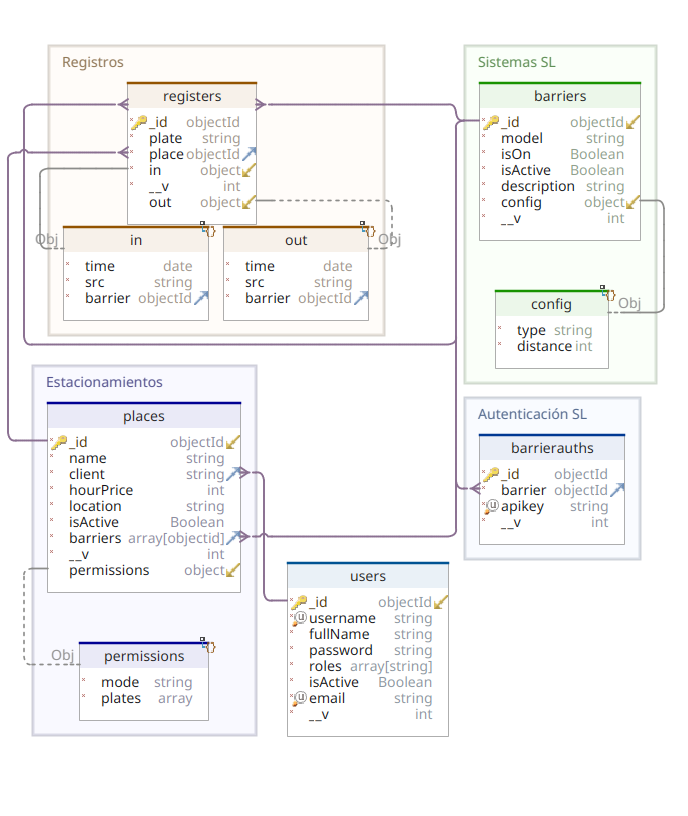
\includegraphics[width=.5\textwidth]{imgs/db.png}
    \caption{Esquema de la base de datos.}
    \label{fig:db-uml}
\end{figure}

\subsection{Broker MQTT}

Un broker MQTT es una aplicación back-end que coordina los mensajes entre los diferentes clientes.
El broker más conocido es Mosquitto, el cual utiliza la versión 5.0 del protocolo. El único tópico implementado tiene la forma de ``\textit{id}/config" donde \textit{id} es un identificador único de los sistemas SL, esto permite que existan tantos tópicos como sistemas SL estén funcionando, y solo pueden escuchar los cambios de configuración de cada una de ellas, lo que permite ahorrar procesamiento de datos en los sistemas SL.

\subsection{Back-end}

El back-end está implementado en NestJS \cite{noauthor_documentacion_nodate}. Su principal función es administrar la información porque se conecta con la base de datos para realizar las tareas de lectura y escritura de documentos.

Con la idea de generar la mayor documentación posible de este servicio se utilizó una librería llamada Swagger la cual, junto a NestJS, genera documentación automática de las rutas HTTP. Esto facilita la tarea de crear una nueva aplicación así como la de incluir una nueva persona al proyecto. En la Fig. \ref{fig:swagger-example} se observa como se ve la documentación generada por Swagger.

\begin{figure}[bth]
    \centering
    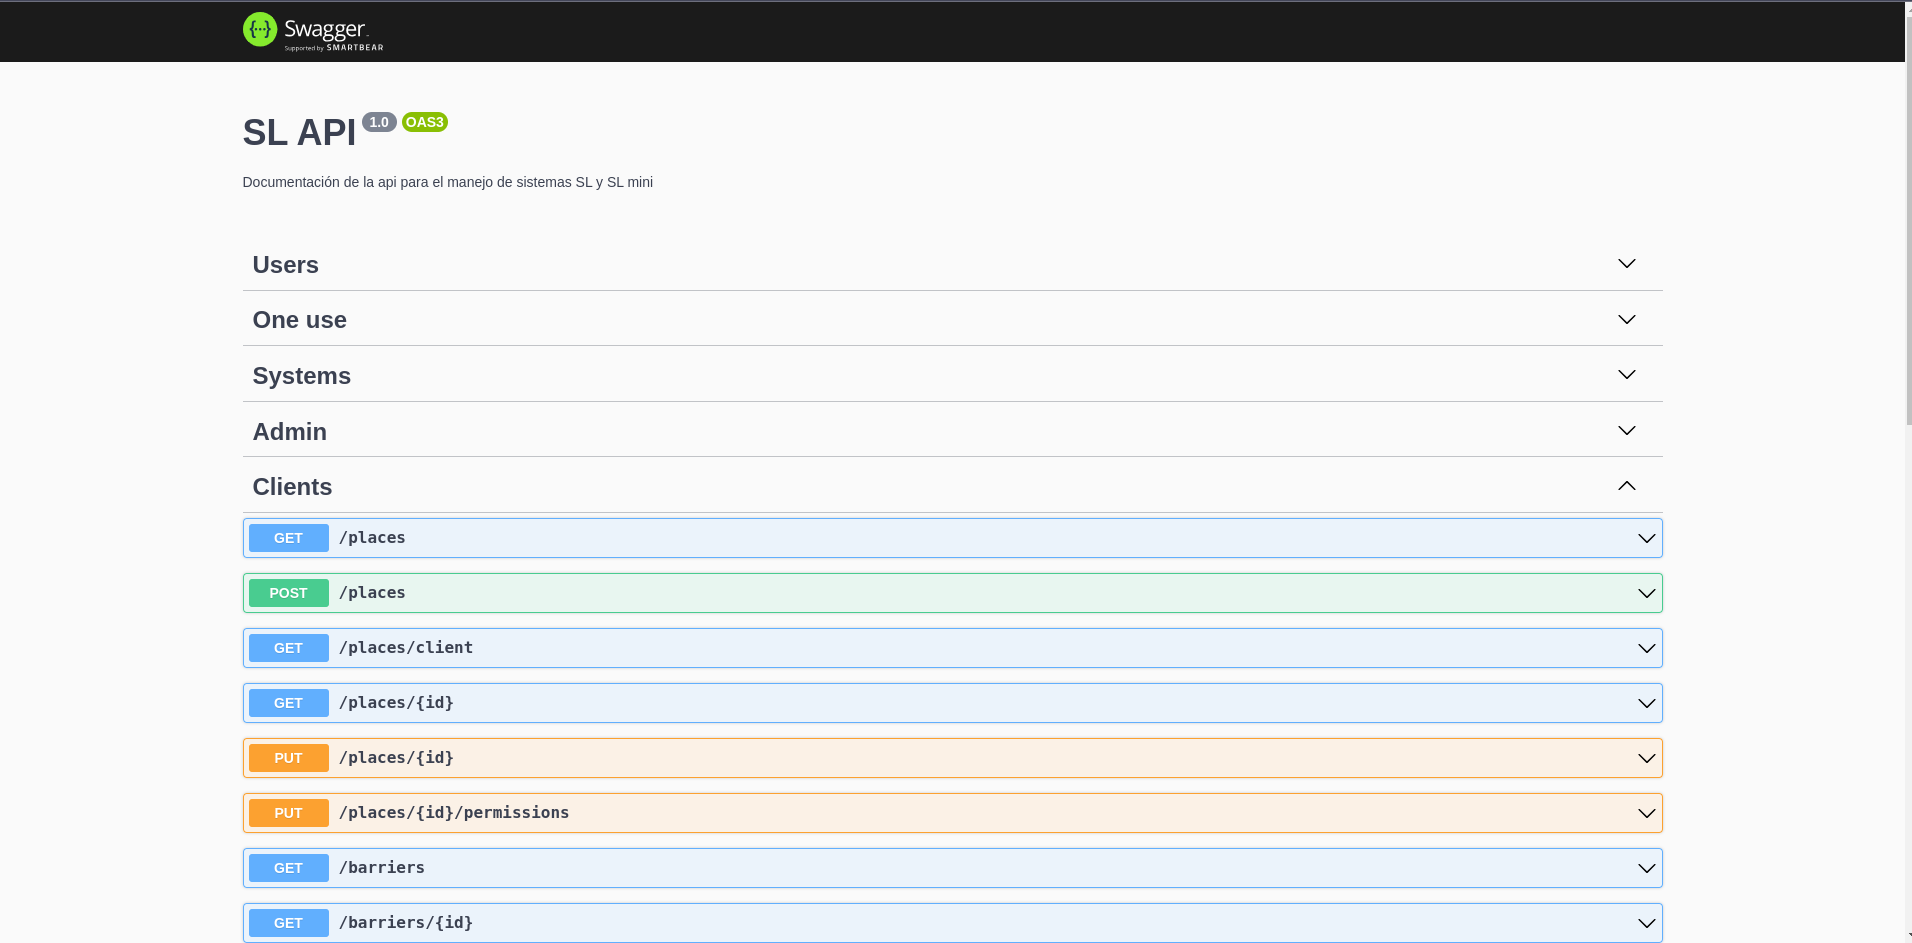
\includegraphics[width=\textwidth]{imgs/server/swagger.png}
    \caption{Documentación generada por Swagger.}
    \label{fig:swagger-example}
\end{figure}

Debido a la necesidad de autenticación de usuarios y de los sistemas SL, se implementó PassportJS que permite la creación de sistemas de validación de forma sencilla. Los métodos de autenticación implementados fueron:

\begin{enumerate}
    \item Usuario y contraseña: Utilizado para los usuarios que entran desde la web.
    \item Api Key de terceros: Una forma de validar si la aplicación que pide datos está autorizada o no.
    \item Api Key para sistemas SL: Permite validar si la información del registro de entrada/salida está siendo enviada por un SL/SL mini autorizado. Además permite saber qué sistema es la que envía los datos, diminuyendo el tamaño de la petición.
    \item Json Web Token o JWT: Se utiliza una vez que el usuario entra a la app, y es un
          hash \footnote{Es el resultado de una operación criptográfica que genera un identificador único e irrepetible a partir de una información dada.}
          generado por el servidor.
\end{enumerate}

\subsubsection{Api Key}

Las Api Key son llaves que generadas en servidor que permiten el accesso a determinados
endpoints \footnote{Son las URLs que consultan desde el front-end.}.
Estas sirven para validar las peticiones entrantes al servidor, permitiendo dar acceso a la información o denegar la consulta HTTP.

\subsubsection{JWT}

JSON Web Token o simplemente JWT es un estándar qué está dentro del documento RFC 7519 \cite{jones_json_2015}. Su función principal es poder propagar información entre dos partes de forma segura. En la práctica, los JWT son muy fáciles de desencriptar por lo que se desaconseja incluir información sensible del usuario en el mismo.

\subsection{Análisis de imágenes}

Este servicio fue implementado con Flask el cual permite crear aplicaciones back-end en Python de forma fácil y rápida. La función de este servicio es obtener la patente de la fotografía tomada por un SL mini, es por ello que solo tiene una ruta e internamente ejecuta el algoritmo visto en el capítulo 3.

\subsection{Front-end}

El front-end fue construido en ReactJS, que es una de las librerías de JavaScript más utilizadas en la industria. La idea principal de este servicio es brindar un centro de control de los sistemas SL, además de permitir la visualización de registros y datos. Además permite a los administradores crear nuevos sistemas SL y visualizar sus parámetros.

\subsubsection{Páginas para los usuarios}

Los usuarios puede registrarse y entrar a la plataforma como se ve en la Fig. \ref{fig:login}. Luego de ingresar pueden visualizar sus estacionamientos (Fig. \ref{fig:home}).

Es posible configurar diversos parámetros del estacionamiento, como el nombre, ubicación y precio por hora (Fig. \ref{fig:update-place}).
Para agregar versatilidad al sistema y permitir su uso para diferentes tareas se implementó un sistema de bloqueo de patentes (Fig. \ref{fig:in-type}), que permite denegar el acceso a  todas las patentes salvo las que estén en la lista o bloquear solo estas últimas. Adicionalmente pueden visualizar los sistemas SL por barrio (Fig. \ref{fig:barrier-details}) y desde esta vista pueden configurar los parámetros de las mismas en tiempo real (Fig. \ref{fig:update-barrier}).

Para la visualización y control de datos se crearon dos rutas.
El Dashboard permite ver información resumida: horas estacionadas y cantidad de vehículos estacionados, separados por estacionamiento, filtrar los datos según fecha de inicio y fin, además permite agrupar los registros día, mes o año (Fig. \ref{fig:dashboard}).
Por otro lado existe una vista de los registros crudos, dando información particular de cada registro (Fig. \ref{fig:registers})


\begin{figure}[!bth]
    \centering
    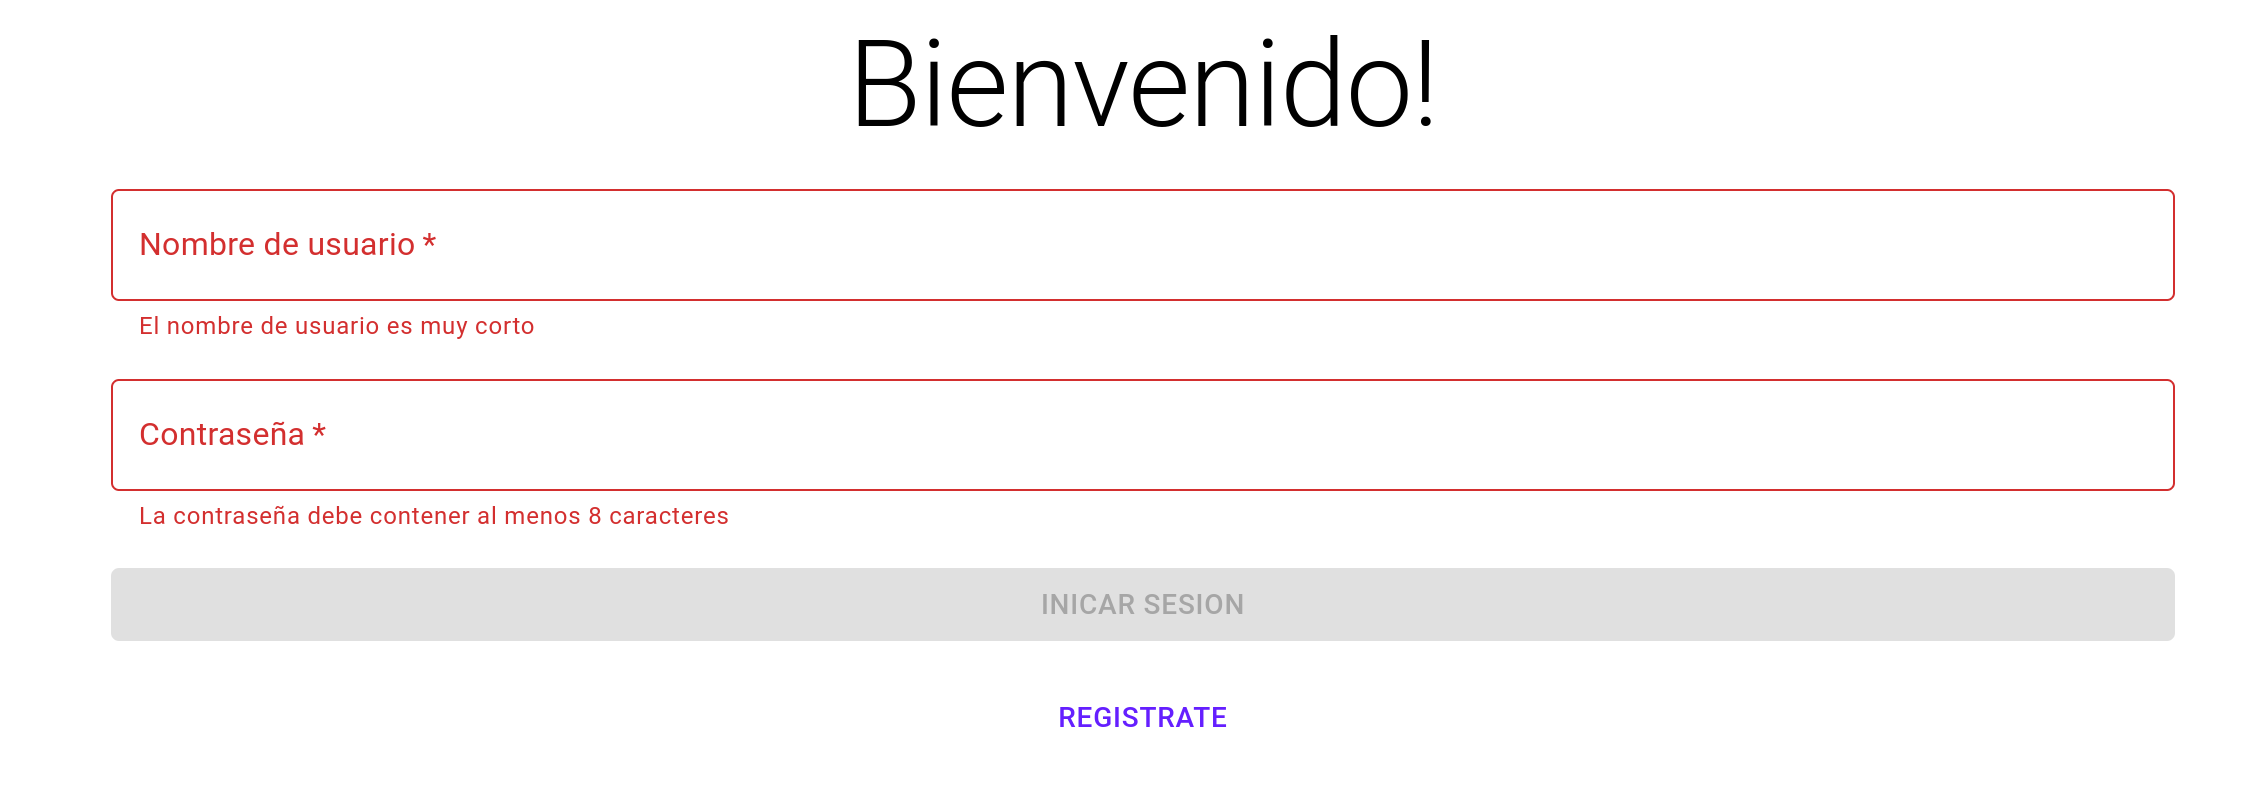
\includegraphics[width=.8\textwidth]{imgs/server/login.png}
    \caption{Inicio de sesión.}
    \label{fig:login}
\end{figure}

\begin{figure}[!bth]
    \centering
    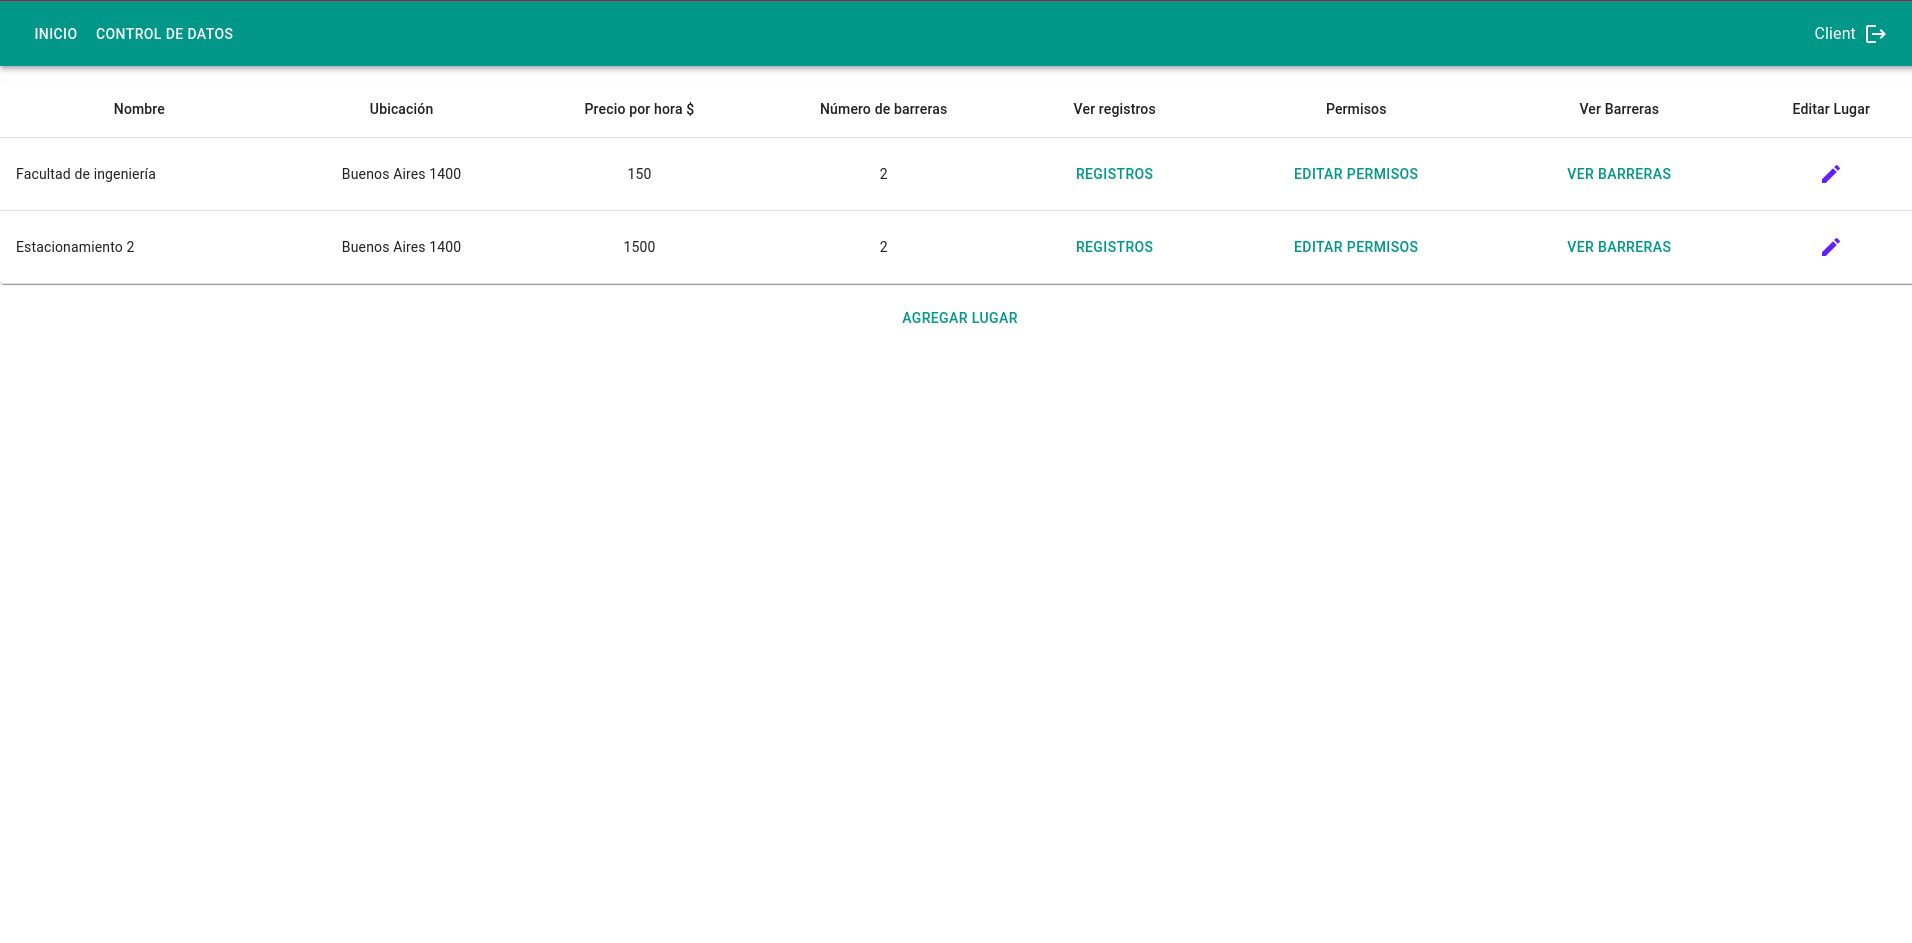
\includegraphics[width=.8\textwidth]{imgs/server/places.png}
    \caption{Estacionamientos del cliente.}
    \label{fig:home}
\end{figure}

\begin{figure}[!bth]
    \centering
    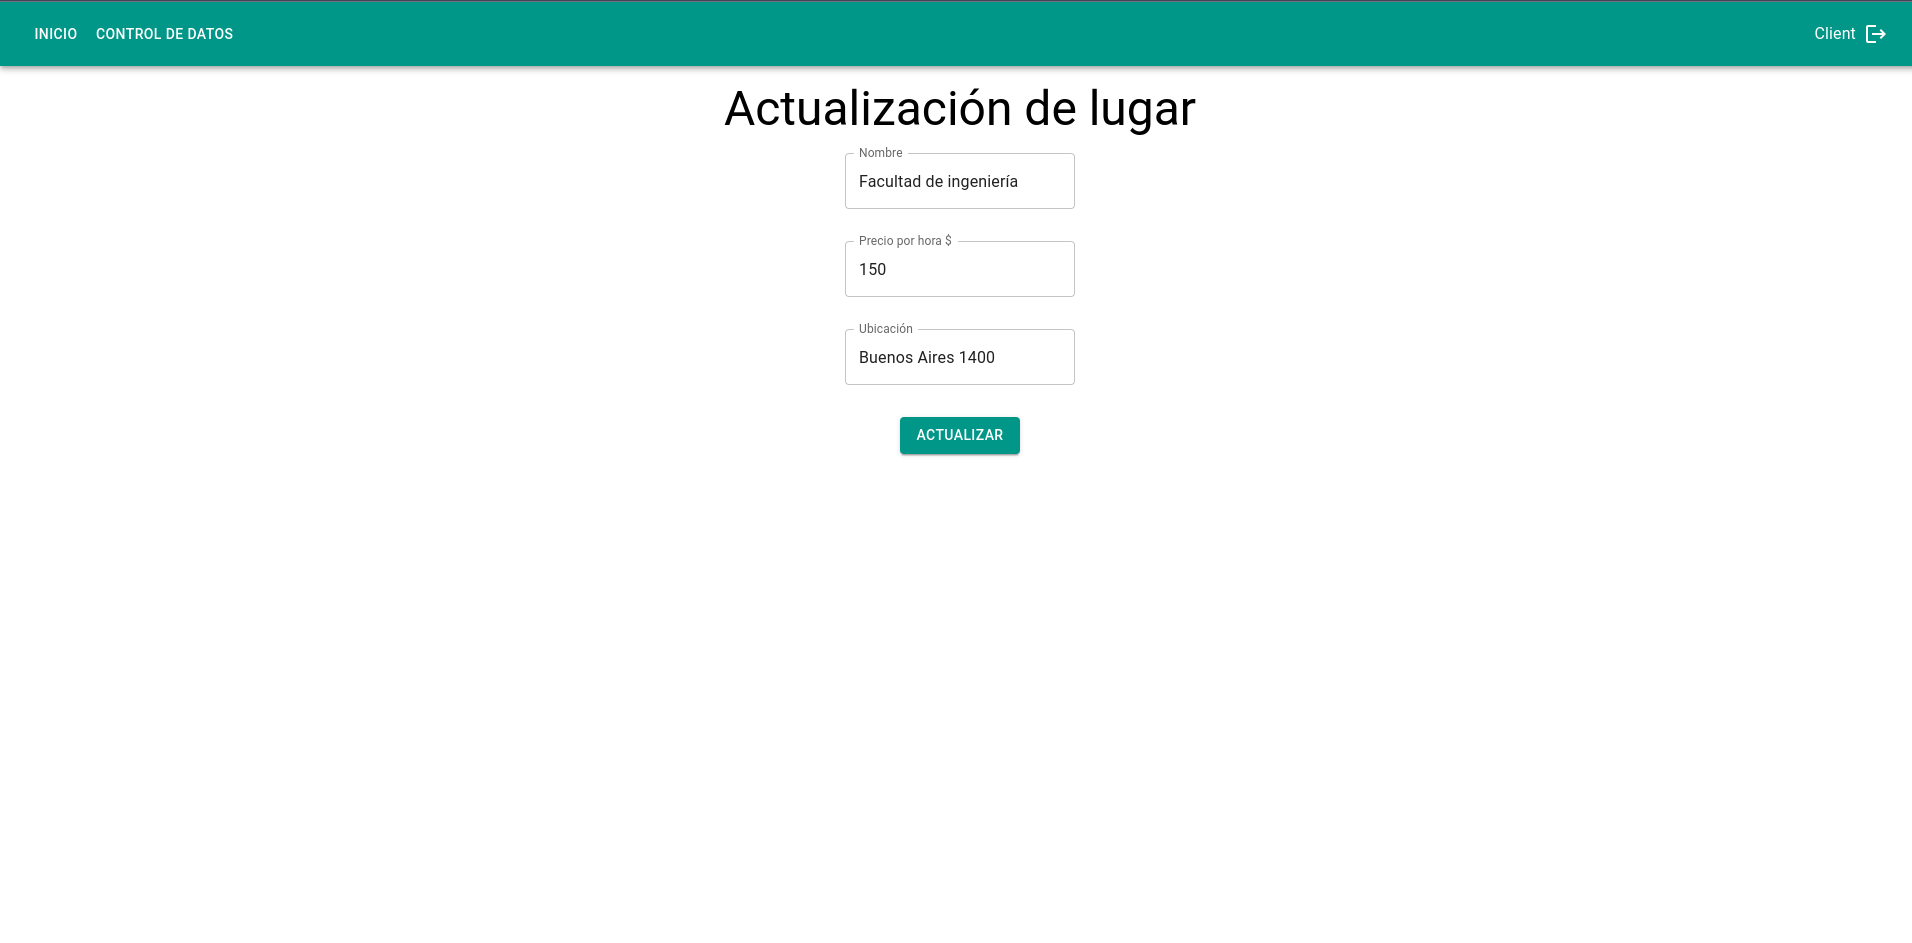
\includegraphics[width=.8\textwidth]{imgs/server/update-place.png}
    \caption{Formulario para actualizar un estacionamiento.}
    \label{fig:update-place}
\end{figure}


\begin{figure}[!bth]
    \centering
    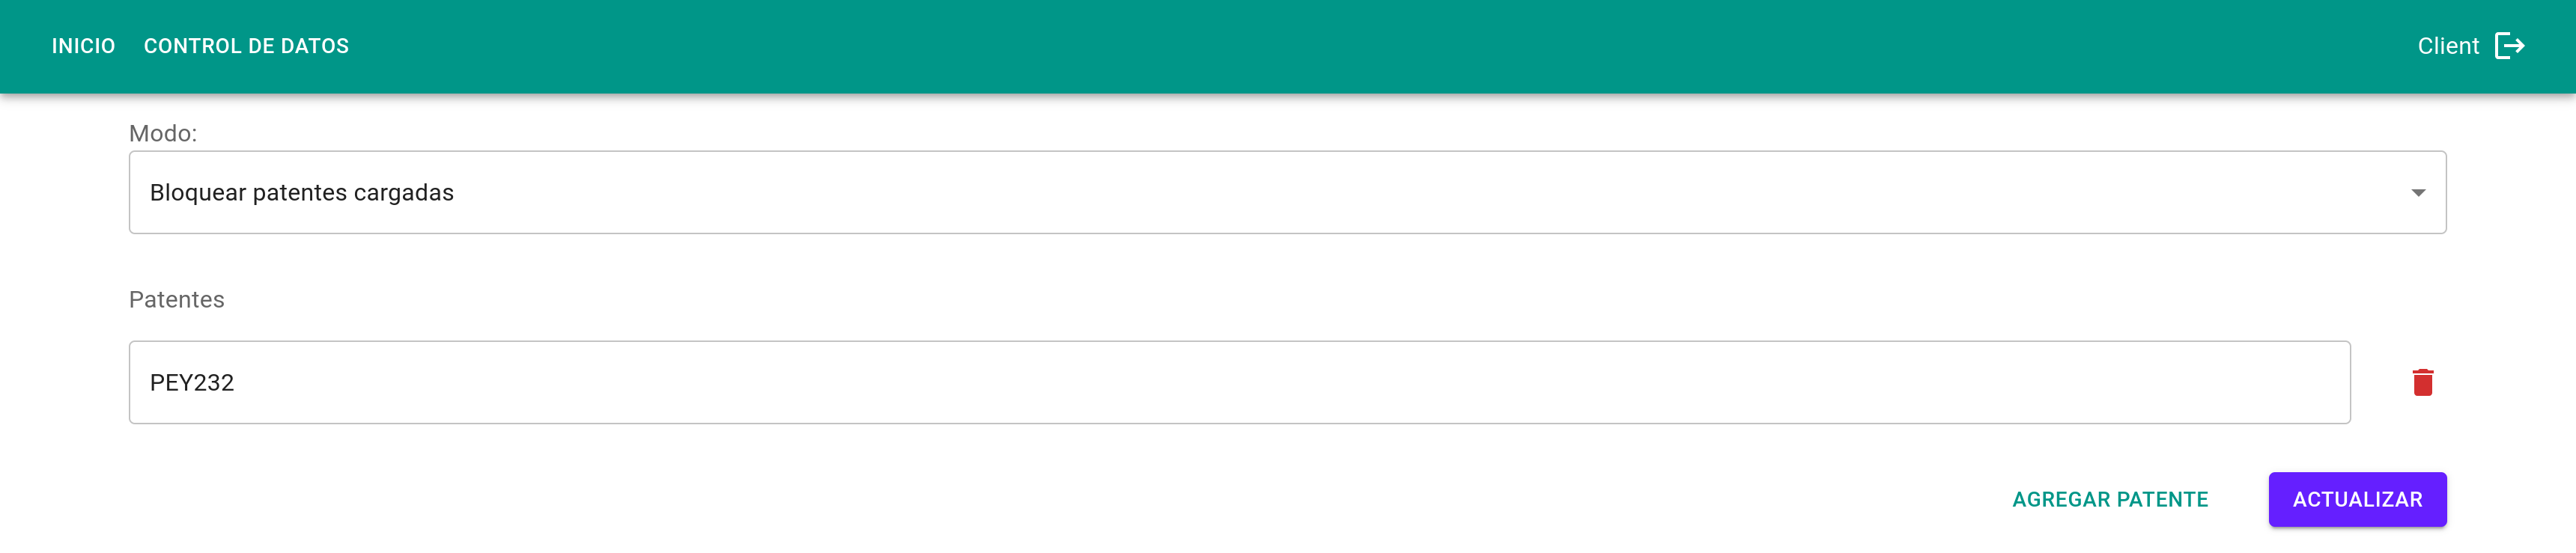
\includegraphics[width=.8\textwidth]{imgs/server/in-type.png}
    \caption{Vista de permisos.}
    \label{fig:in-type}
\end{figure}
\begin{figure}[!bth]
    \centering
    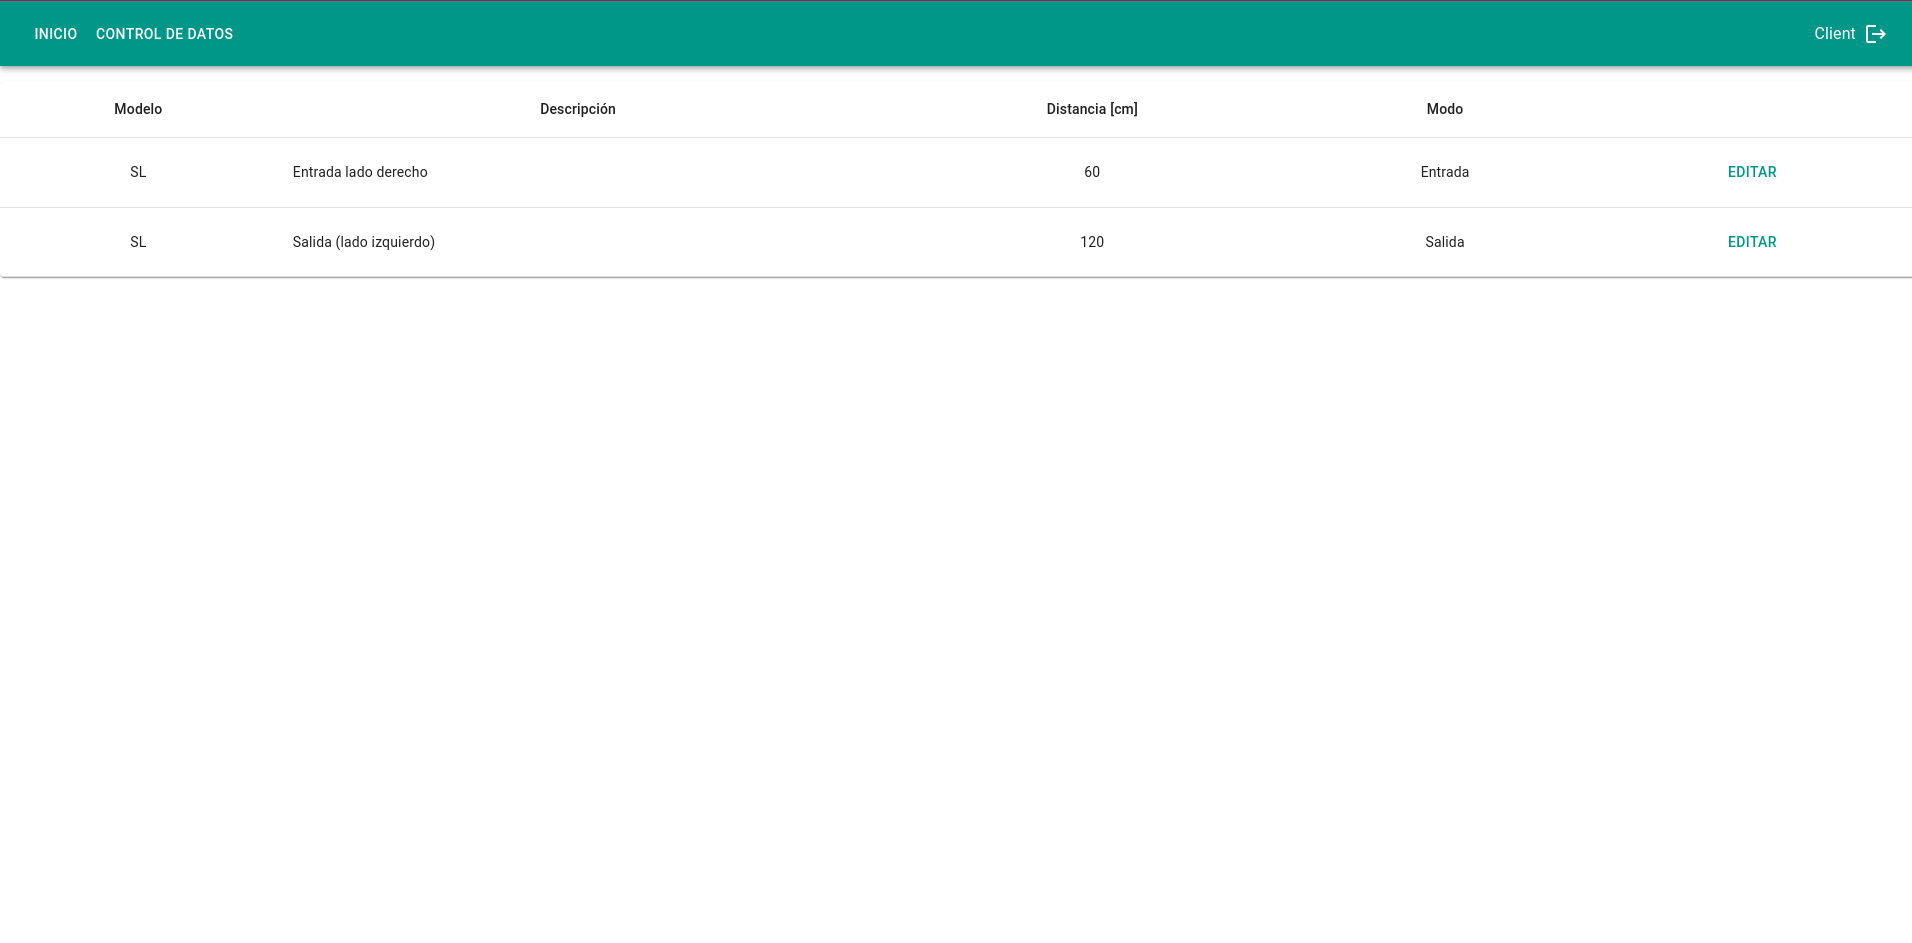
\includegraphics[width=.8\textwidth]{imgs/server/client-barriers-details.png}
    \caption{Vista de los detalles.}
    \label{fig:barrier-details}
\end{figure}

\begin{figure}[!bth]
    \centering
    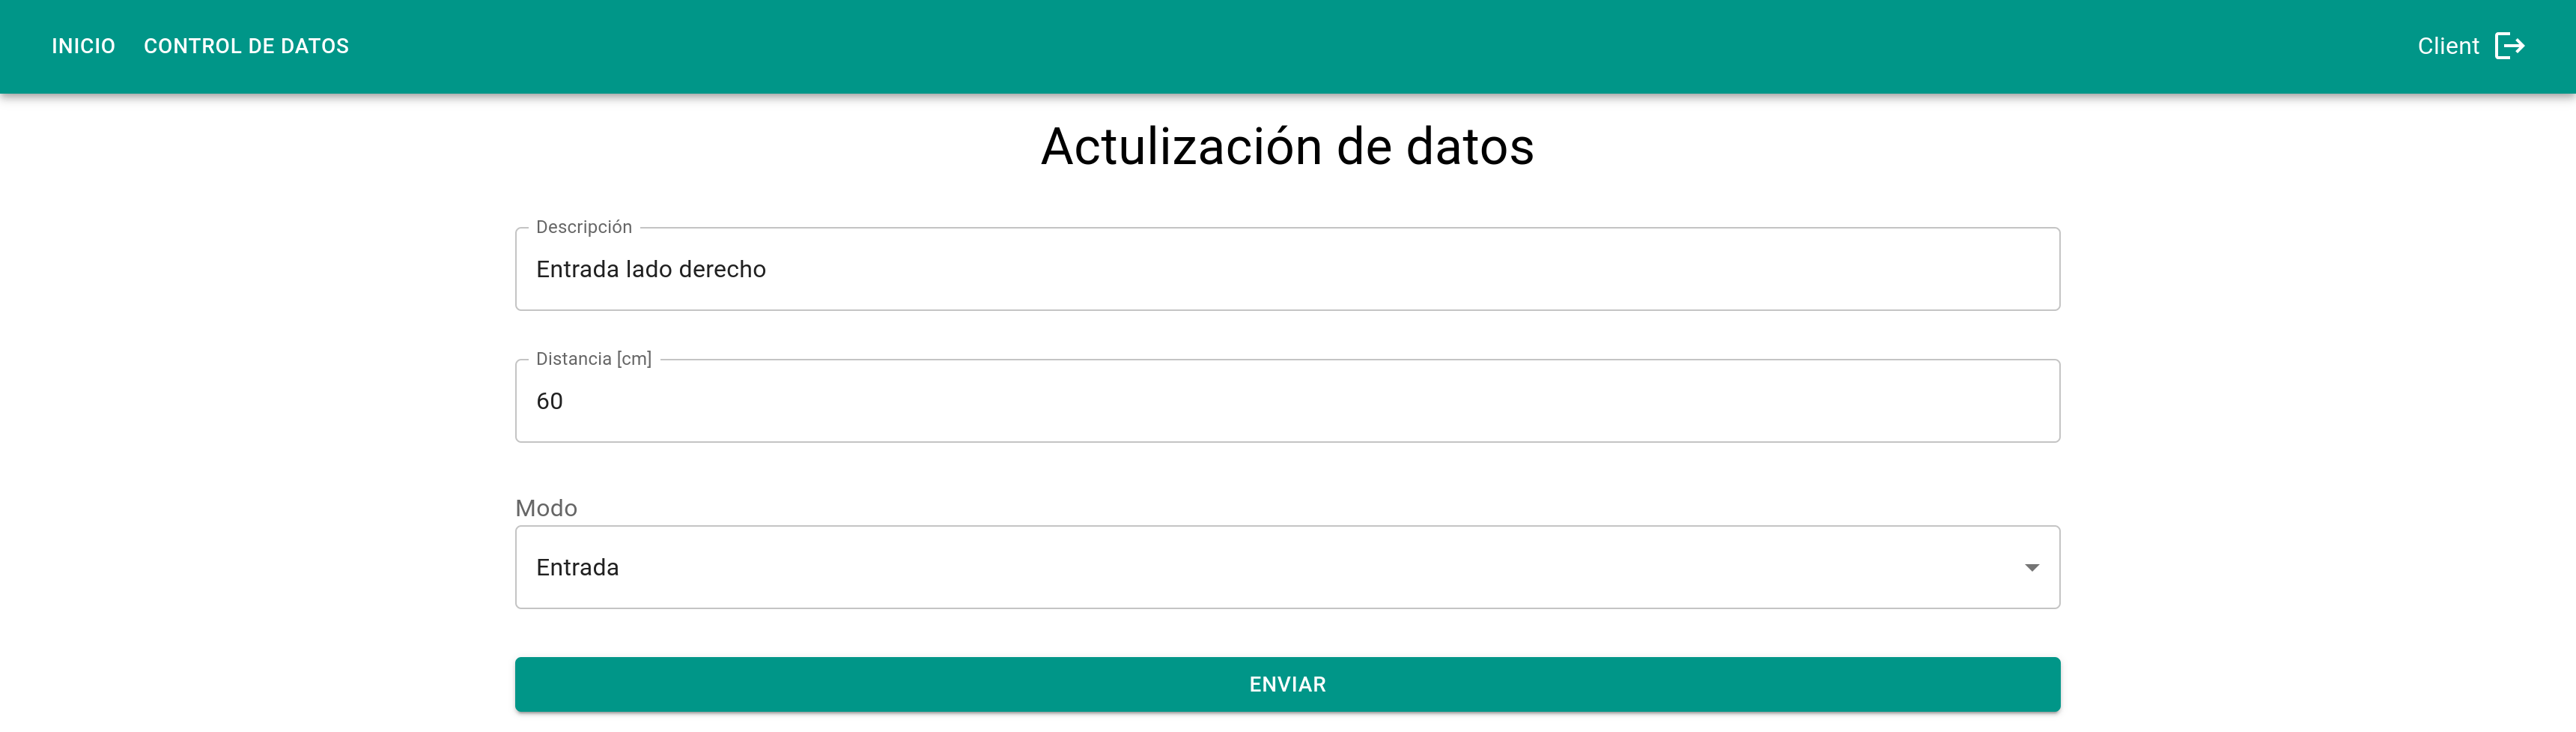
\includegraphics[width=.8\textwidth]{imgs/server/barrier-update-data.png}
    \caption{Formulario para actualizar los datos del sistema SL.}
    \label{fig:update-barrier}
\end{figure}

\begin{figure}[!bth]
    \centering
    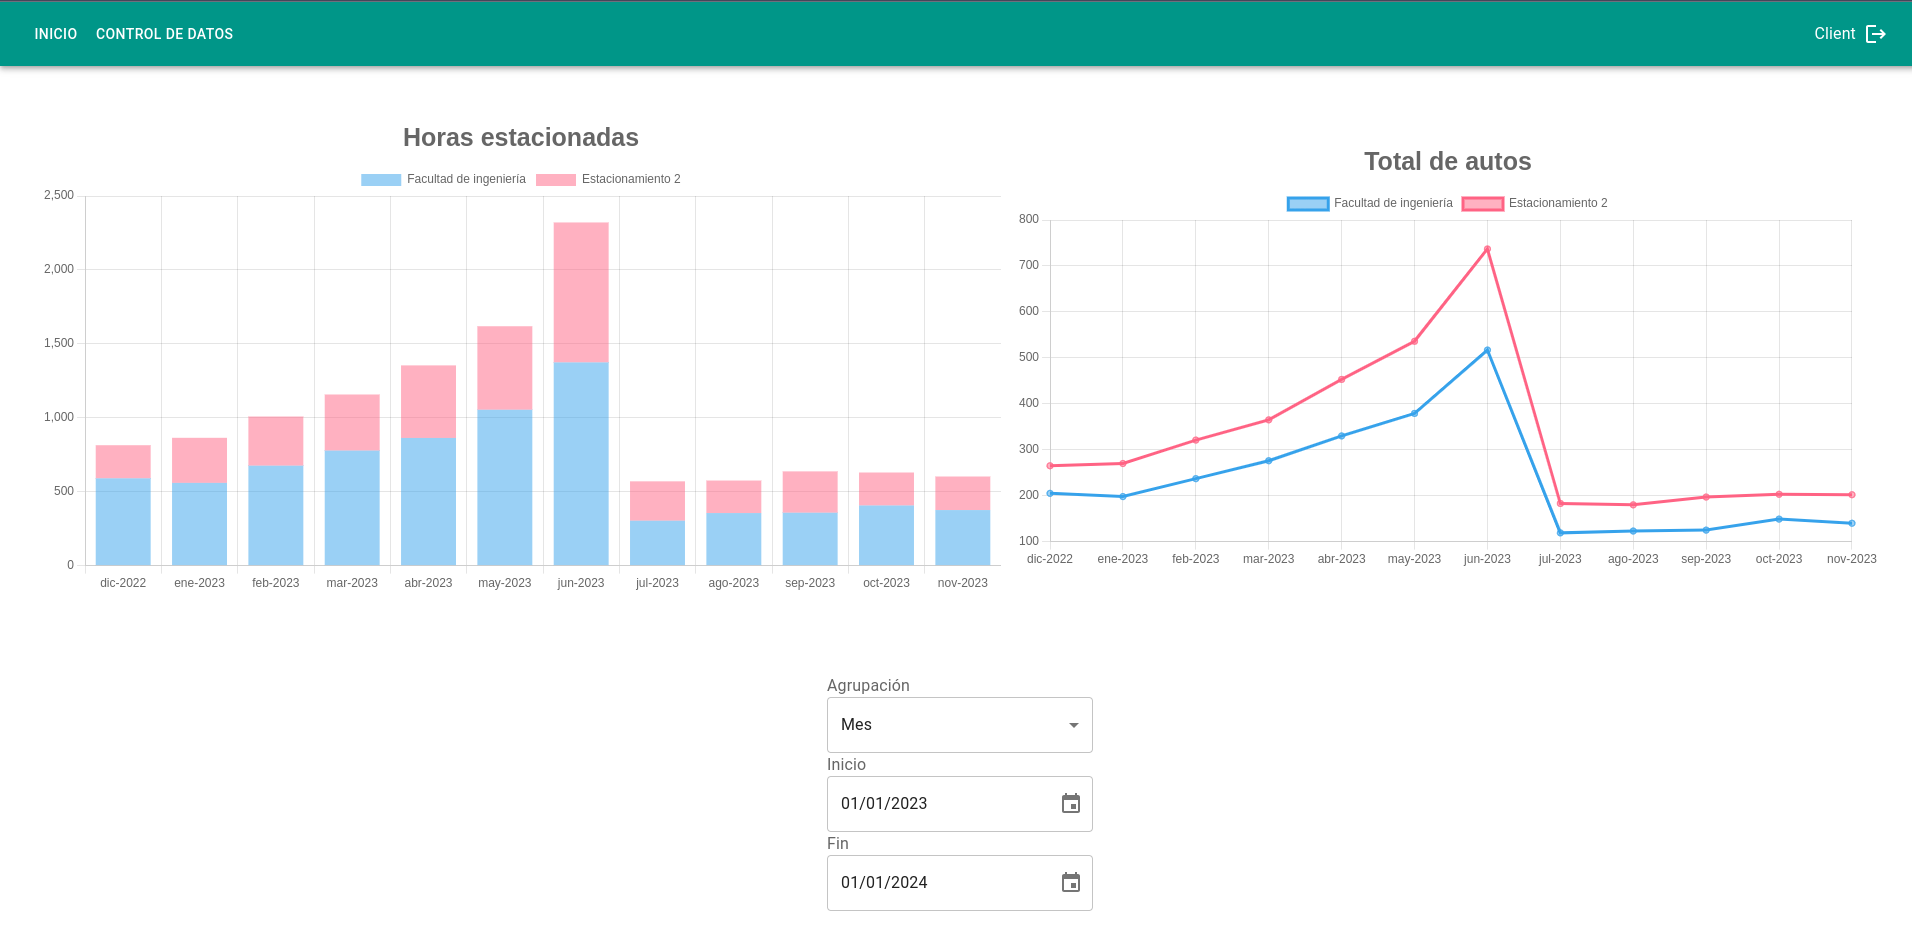
\includegraphics[width=.8\textwidth]{imgs/server/resume.png}
    \caption{Visualización de datos para un cliente con 2 estacionamientos.}
    \label{fig:dashboard}
\end{figure}

\begin{figure}[!bth]
    \centering
    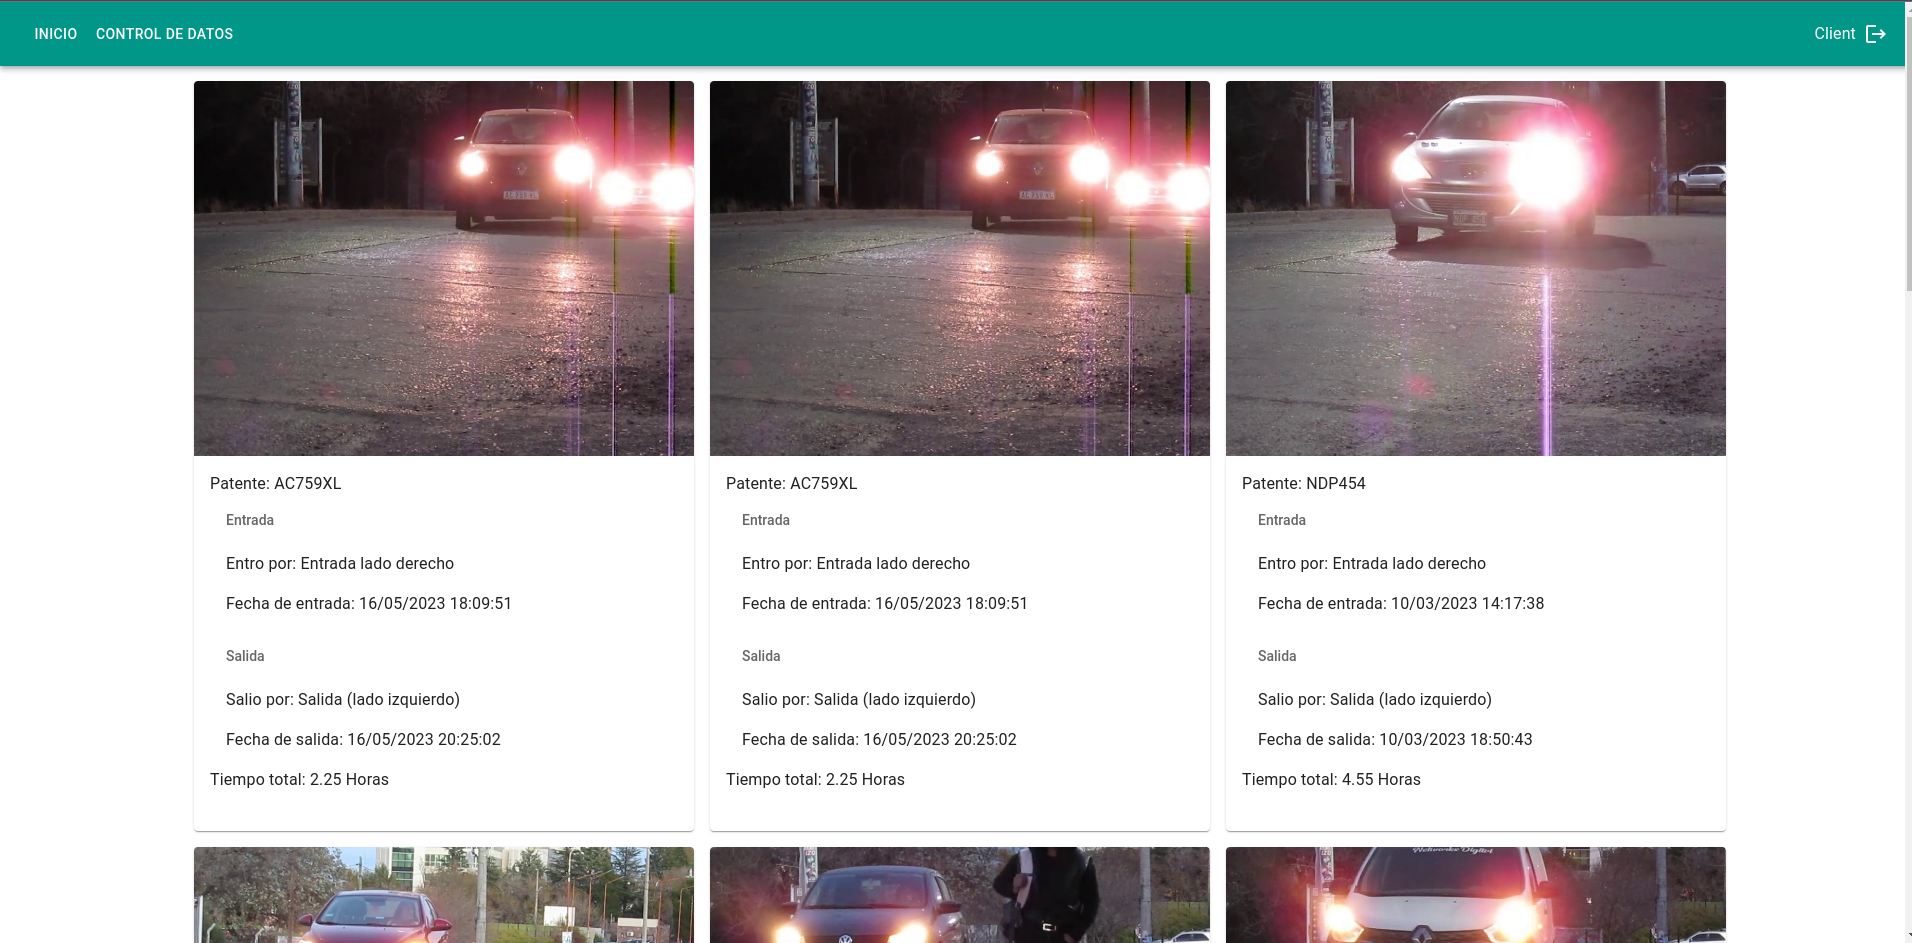
\includegraphics[width=.8\textwidth]{imgs/server/registers.png}
    \caption{Vista de registros.}
    \label{fig:registers}
\end{figure}



\subsubsection{Páginas para los administradores}

Los administradores poseen una página para visualizar los sistemas SL según cliente y lugar (Fig. \ref{fig:admin-details}). Por último, poseen una página para agregar sistemas SL (Fig. \ref{fig:add-barrier}).

\begin{figure}[!bth]
    \centering
    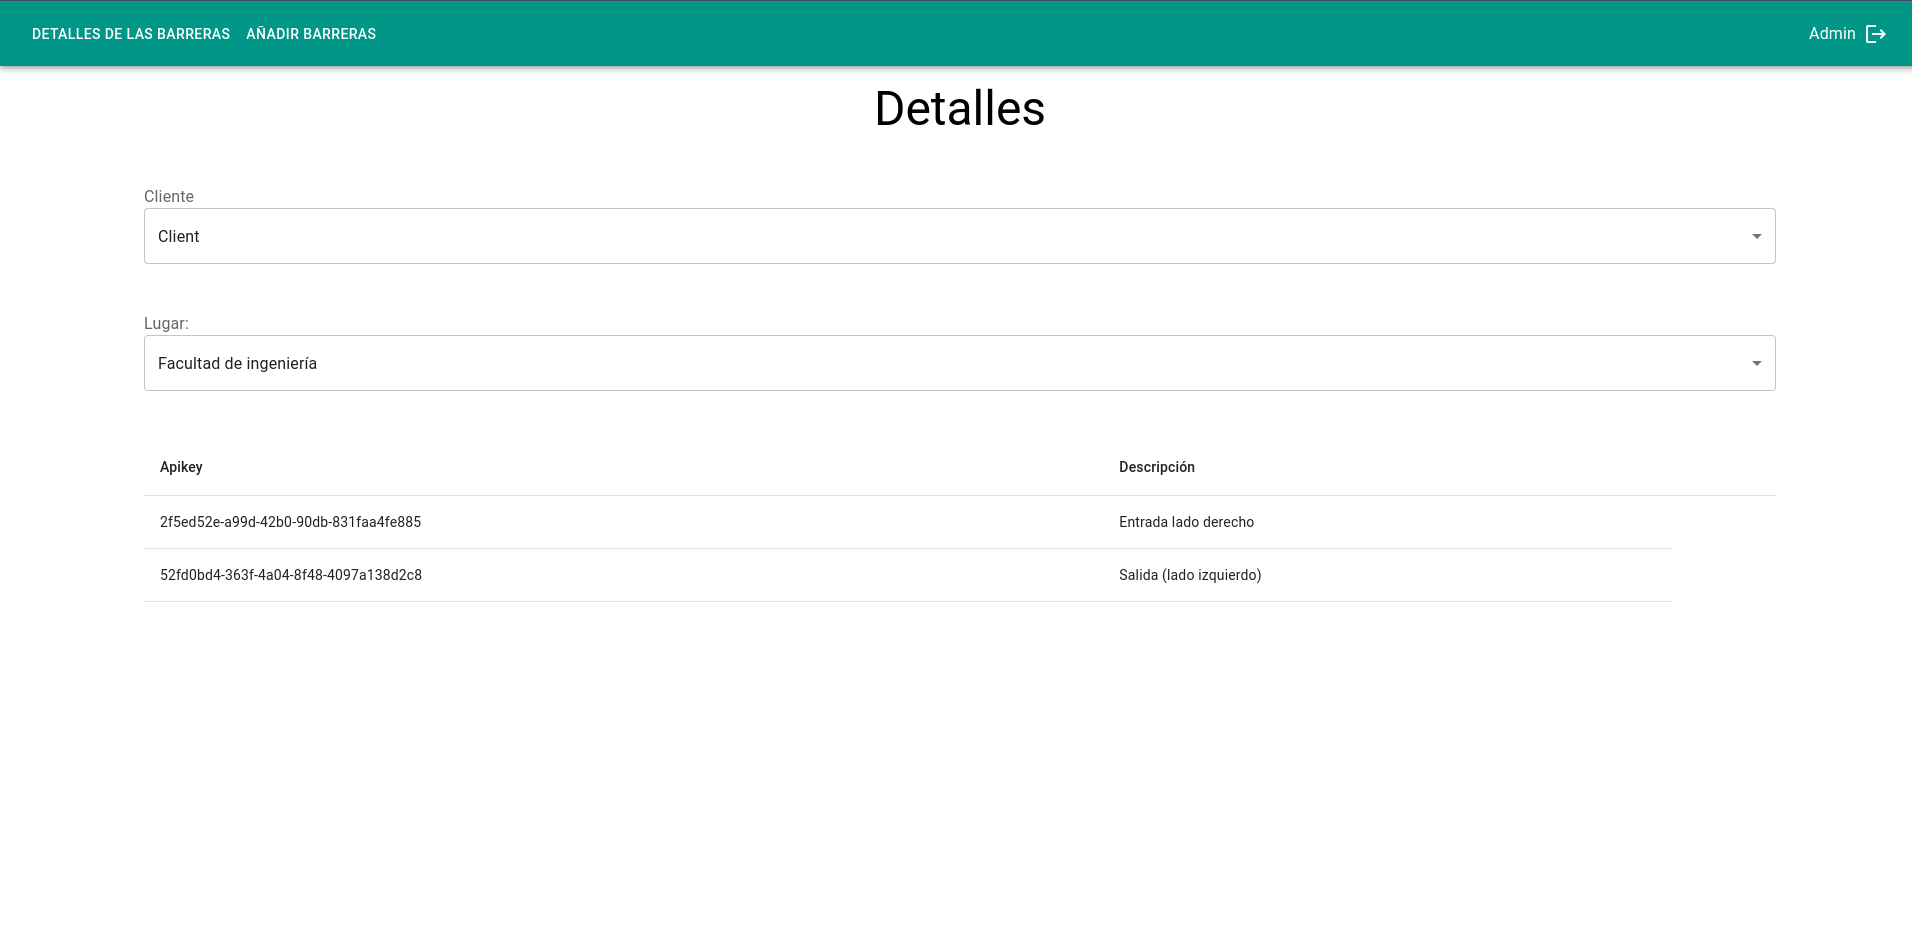
\includegraphics[width=.8\textwidth]{imgs/server/admin-details.png}
    \caption{Detalles de los sistemas SL según cliente y estacionamiento.}
    \label{fig:admin-details}
\end{figure}

\begin{figure}[!bth]
    \centering
    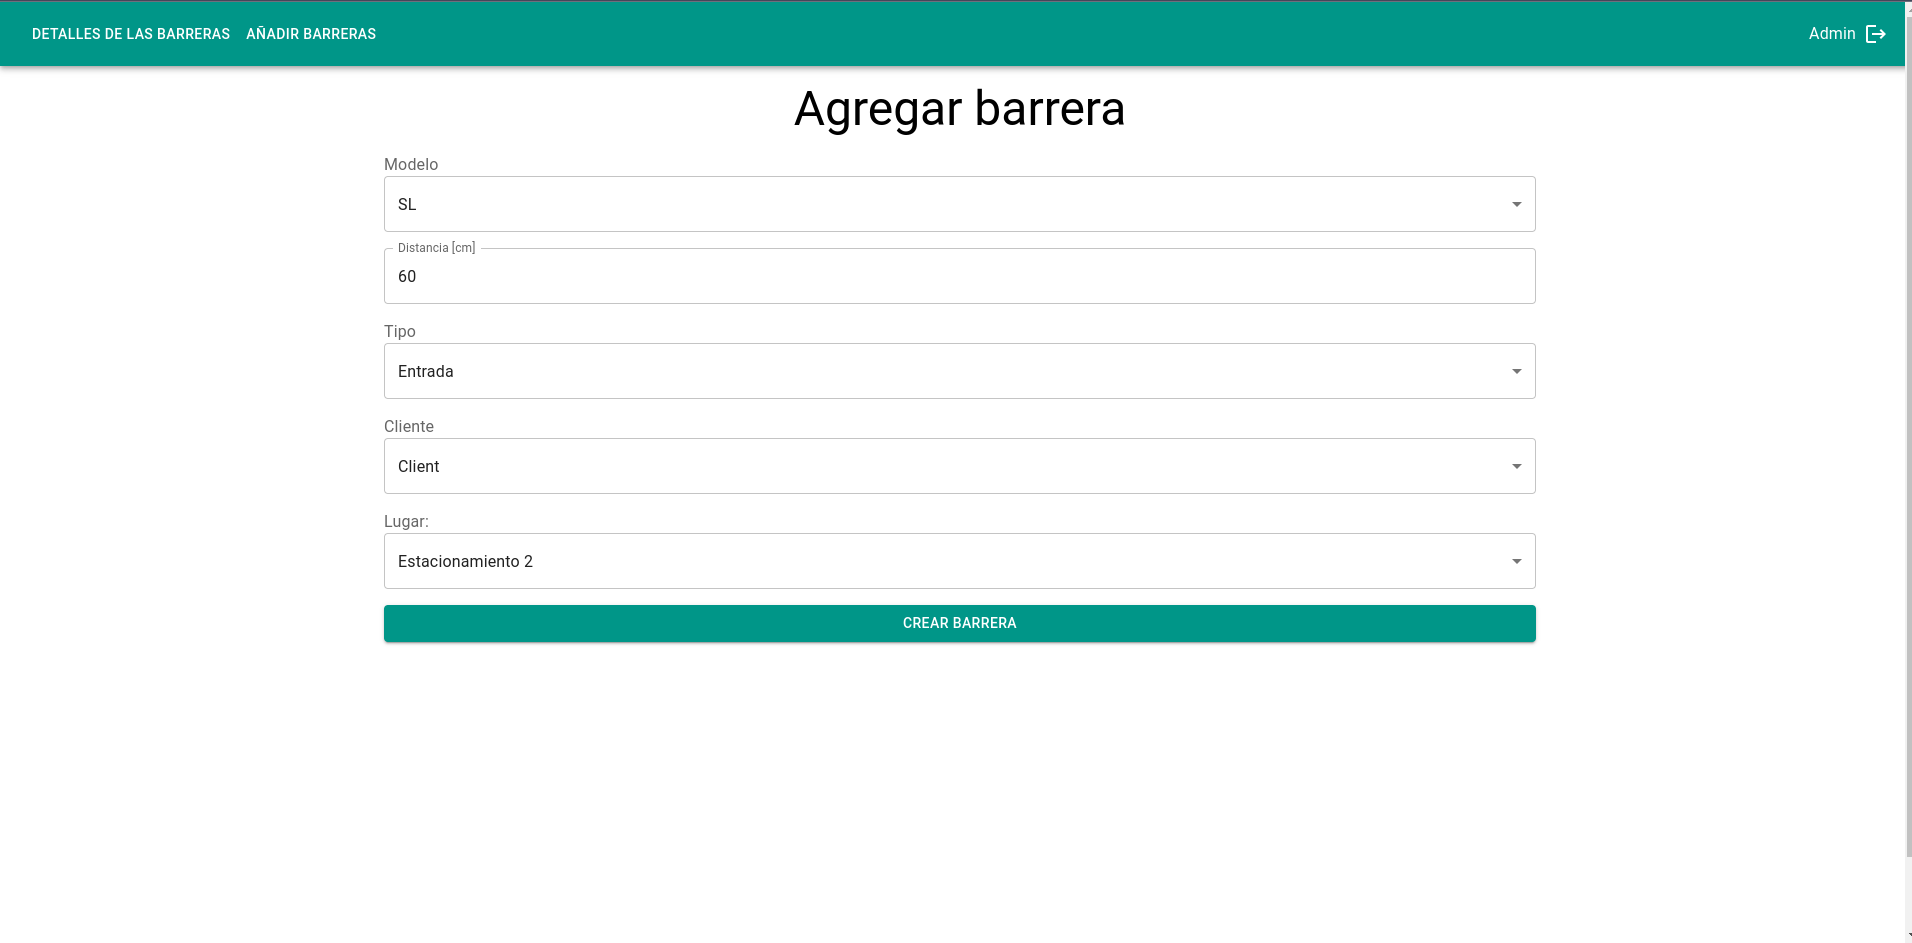
\includegraphics[width=.8\textwidth]{imgs/server/add-barrier.png}
    \caption{Formulario para agregar un sistema SL.}
    \label{fig:add-barrier}
\end{figure}

\subsection{Nginx}

Nginx es un servidor web de código abierto que permite la implementación de
proxy inverso\footnote{Es una aplicación back-end que se situa delante de otros servicios web, aumentando la seguridad, el rendimiendo y la fiabilidad del servidor.}, cache de HTTP, y balanceo de cargo.
Su implementación se utiliza como proxy inverso entre el back-end y el front-end.



